\documentclass[11pt]{preprint}

\setlength{\topmargin}{0mm} \setlength{\oddsidemargin}{0mm}
\setlength{\textwidth}{160mm} \setlength{\textheight}{215mm}

\usepackage{amssymb,amsmath,amscd,amsthm}
\usepackage{graphics}
\usepackage{tikz}

\def\enumb{\begin{enumerate}}
\def\enume{\end{enumerate}}
\def\itemb{\begin{itemize}}
\def\iteme{\end{itemize}}
\def\integers{\mathbb{Z}}

\def\multiset#1#2{\ensuremath{\left(\kern-.3em\left(\genfrac{}{}{0pt}{}{#1}{#2}\right)\kern-.3em\right)}}



\newtheorem{proposition}{Proposition}
\newtheorem{theorem}{Theorem}

\title{Discrete Mathematics, 2016 Fall - Worksheet 23}
\author{Instructor: Zsolt Pajor-Gyulai, CIMS}



\begin{document}

\maketitle

In all of the above problems explain your answer in full English sentences.

\enumb
\item Let $G$ be the graph in the figure.
\begin{figure}[ht]
\centering
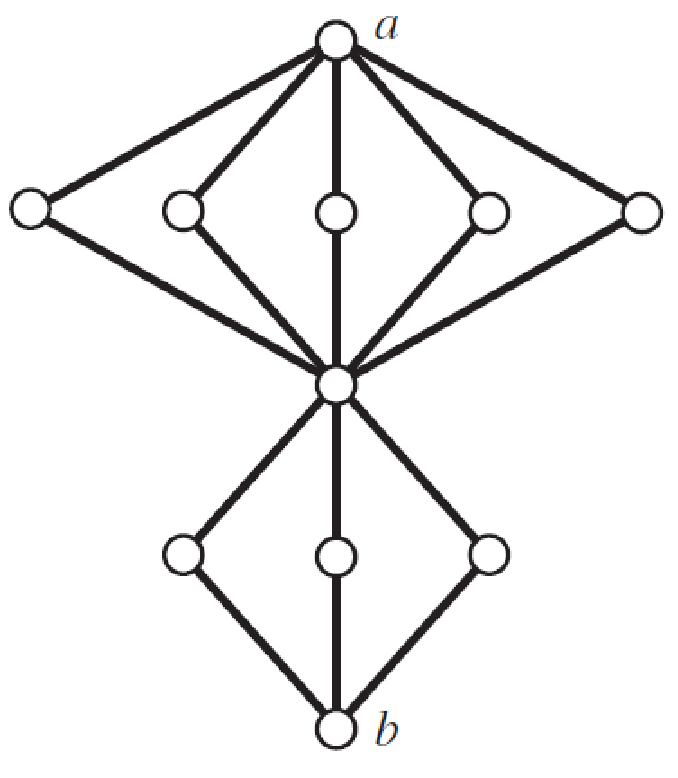
\includegraphics[scale=0.3]{WS1.pdf}
\end{figure}
\enumb
\item How many different paths are there from $a$ to $b$?
\item How many different walks are there from $a$ to $b$?
\enume
\item Prove that $K_n$ is connected.
\item Suppose $G$ is a connected graph in which each vertex has even degree. Then, $G$ has no cut edges.
\item List all the trees
\enumb
\item with vertex set $\{1,2,3\}$
\item with vertex set $\{1,2,3,4\}$
\enume
\item 
\begin{enumerate}
\item[a)] Let $T$ be a tree with $n\geq 1$ vertices. Prove that $T$ has $n-1$ edges.


\item[b)] Prove the converse, i.e. that if $G$ is a connected graph that has exactly $n-1$ edges then $G$ must be a tree.


\end{enumerate}
\item Let $T$ be a tree. Prove that the average degree of a vertex in $T$ is less than $2$.



\enume
\end{document}